% vim: set spell spelllang=en tw=100 et sw=4 sts=4 foldmethod=marker foldmarker={{{,}}} :

\documentclass{beamer}

\usepackage{etex}
\usepackage{tikz}
\usepackage{xcolor}
\usepackage{complexity}
\usepackage{hyperref}
\usepackage{microtype}
\usepackage{amsmath}                   % \operatorname
\usepackage{amsfonts}                  % \mathcal
\usepackage{amssymb}                   % \nexists
\usepackage{gnuplot-lua-tikz}          % graphs
\usepackage[vlined]{algorithm2e} % algorithms
\usepackage{centernot}
\usepackage{mathtools}
\usepackage{listings}
\usepackage{chemfig}

\usetikzlibrary{shapes, arrows, shadows, calc, positioning, fit}
\usetikzlibrary{decorations.pathreplacing, decorations.pathmorphing, shapes.misc}
\usetikzlibrary{tikzmark}

\definecolor{uofguniversityblue}{rgb}{0, 0.219608, 0.396078}

\definecolor{uofgheather}{rgb}{0.356863, 0.32549, 0.490196}
\definecolor{uofgaquamarine}{rgb}{0.603922, 0.72549, 0.678431}
\definecolor{uofgslate}{rgb}{0.309804, 0.34902, 0.380392}
\definecolor{uofgrose}{rgb}{0.823529, 0.470588, 0.709804}
\definecolor{uofgmocha}{rgb}{0.709804, 0.564706, 0.47451}
\definecolor{uofgsandstone}{rgb}{0.321569, 0.278431, 0.231373}
\definecolor{uofgforest}{rgb}{0, 0.2, 0.129412}
\definecolor{uofglawn}{rgb}{0.517647, 0.741176, 0}
\definecolor{uofgcobalt}{rgb}{0, 0.615686, 0.92549}
\definecolor{uofgturquoise}{rgb}{0, 0.709804, 0.819608}
\definecolor{uofgsunshine}{rgb}{1.0, 0.862745, 0.211765}
\definecolor{uofgpumpkin}{rgb}{1.0, 0.72549, 0.282353}
\definecolor{uofgthistle}{rgb}{0.584314, 0.070588, 0.447059}
\definecolor{uofgrust}{rgb}{0.603922, 0.227451, 0.023529}
\definecolor{uofgburgundy}{rgb}{0.490196, 0.133333, 0.223529}
\definecolor{uofgpillarbox}{rgb}{0.701961, 0.047059, 0}
\definecolor{uofglavendar}{rgb}{0.356863, 0.301961, 0.580392}

\tikzset{vertex/.style={draw, circle, inner sep=0pt, minimum size=0.5cm, font=\small\bfseries}}
\tikzset{notvertex/.style={vertex, color=white, text=black}}
\tikzset{plainvertex/.style={vertex}}
\tikzset{vertexc1/.style={vertex, fill=uofgcobalt}}
\tikzset{vertexc2/.style={vertex, fill=uofglawn}}
\tikzset{vertexc3/.style={vertex, fill=uofgpumpkin}}
\tikzset{vertexc4/.style={vertex, fill=uofgheather}}
\tikzset{edge/.style={color=black!50!white}}
\tikzset{bedge/.style={ultra thick}}
\tikzset{edged/.style={color=screengrey, dashed}}
\tikzset{edgel3/.style={color=uofgthistle, ultra thick}}

\newcommand*\circled[1]{\tikz[baseline=(char.base)]{
            \node[shape=circle,draw,inner sep=0pt] (char) {#1};}}

% {{{ theme things
\useoutertheme[footline=authortitle]{miniframes}
\useinnertheme{rectangles}

\setbeamerfont{block title}{size={}}
\setbeamerfont{title}{size=\large,series=\bfseries}
\setbeamerfont{section title}{size=\large,series=\mdseries}
\setbeamerfont{author}{size=\normalsize,series=\mdseries}
\setbeamercolor*{structure}{fg=uofguniversityblue}
\setbeamercolor*{palette primary}{use=structure,fg=black,bg=white}
\setbeamercolor*{palette secondary}{use=structure,fg=white,bg=uofgcobalt}
\setbeamercolor*{palette tertiary}{use=structure,fg=white,bg=uofguniversityblue}
\setbeamercolor*{palette quaternary}{fg=white,bg=black}

\setbeamercolor*{titlelike}{parent=palette primary}

\beamertemplatenavigationsymbolsempty

\setbeamertemplate{title page}
{
    \begin{tikzpicture}[remember picture, overlay]
        \node at (current page.north west) {
            \begin{tikzpicture}[remember picture, overlay]
                \fill [fill=uofguniversityblue, anchor=north west] (0, 0) rectangle (\paperwidth, -2.6cm);
            \end{tikzpicture}
        };

        \node (logo) [anchor=north east, shift={(-0.6cm,-0.6cm)}] at (current page.north east) {
            \includegraphics*[keepaspectratio=true,scale=0.7]{UoG_keyline.pdf}
        };

        \node [anchor=west, xshift=0.2cm] at (current page.west |- logo.west) {
            \begin{minipage}{0.65\paperwidth}\raggedright
                {\usebeamerfont{title}\usebeamercolor[white]{}\inserttitle}\\[0.1cm]
                {\usebeamerfont{author}\usebeamercolor[white]{}\insertauthor}
            \end{minipage}
        };
    \end{tikzpicture}
}

\setbeamertemplate{section page}
{
    \begin{centering}
        \begin{beamercolorbox}[sep=12pt,center]{part title}
            \usebeamerfont{section title}\insertsection\par
        \end{beamercolorbox}
    \end{centering}
}

\newcommand{\frameofframes}{/}
\newcommand{\setframeofframes}[1]{\renewcommand{\frameofframes}{#1}}

\makeatletter
\setbeamertemplate{footline}
{%
    \begin{beamercolorbox}[colsep=1.5pt]{upper separation line foot}
    \end{beamercolorbox}
    \begin{beamercolorbox}[ht=2.5ex,dp=1.125ex,%
        leftskip=.3cm,rightskip=.3cm plus1fil]{author in head/foot}%
        \leavevmode{\usebeamerfont{author in head/foot}\insertshortauthor}%
        \hfill%
        {\usebeamerfont{institute in head/foot}\usebeamercolor[fg]{institute in head/foot}\insertshortinstitute}%
    \end{beamercolorbox}%
    \begin{beamercolorbox}[ht=2.5ex,dp=1.125ex,%
        leftskip=.3cm,rightskip=.3cm plus1fil]{title in head/foot}%
        {\usebeamerfont{title in head/foot}\insertshorttitle}%
        \hfill%
        {\usebeamerfont{frame number}\usebeamercolor[fg]{frame number}\insertframenumber~\frameofframes~\inserttotalframenumber}
    \end{beamercolorbox}%
    \begin{beamercolorbox}[colsep=1.5pt]{lower separation line foot}
    \end{beamercolorbox}
}

% }}}

\title[Solving Hard Graph Problems in Parallel]{Solving Hard Graph Problems \\ in Parallel}
\author[Ciaran McCreesh and Patrick Prosser]{\textbf{Ciaran McCreesh} and Patrick Prosser}

\begin{document}

{
    \usebackgroundtemplate{
        \tikz[overlay, remember picture]
        \node[at=(current page.south), anchor=south, inner sep=0pt]{\includegraphics*[keepaspectratio=true, width=\paperwidth]{background.jpg}};
    }
    \begin{frame}[plain,noframenumbering]
        \titlepage
    \end{frame}
}

\section{\ldots{}Hard Graph Problems\ldots}

\begin{frame}{The Maximum Clique Problem}
    \begin{center}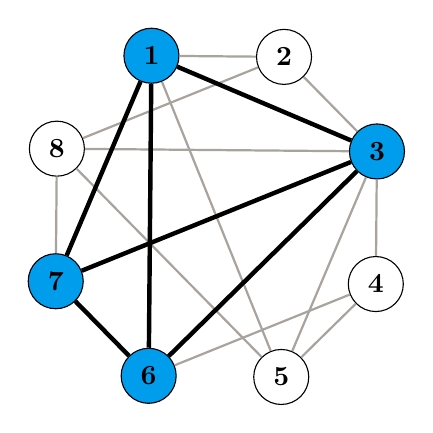
\begin{tikzpicture}
        \newcount \c
        \foreach \n in {1, ..., 8}{
            \c=\n \advance\c by -1 \multiply\c by -360 \divide\c by 8 \advance\c by 112.5
            \ifthenelse{\n = 1 \OR \n = 3 \OR \n = 6 \OR \n = 7}{
                \node[draw, circle, fill=uofgcobalt, inner sep=4pt, font=\bfseries] (N\n) at (\the\c:2.2) {\n};
            }{
                \node[draw, circle, fill=white, inner sep=4pt, font=\bfseries] (N\n) at (\the\c:2.2) {\n};
            }
        }

        \draw [thick, color=uofgsandstone!50] (N1) -- (N2);
        \draw [thick, color=uofgsandstone!50] (N1) -- (N5);
        \draw [thick, color=uofgsandstone!50] (N2) -- (N3);
        \draw [thick, color=uofgsandstone!50] (N2) -- (N8);
        \draw [thick, color=uofgsandstone!50] (N3) -- (N4);
        \draw [thick, color=uofgsandstone!50] (N3) -- (N5);
        \draw [thick, color=uofgsandstone!50] (N3) -- (N8);
        \draw [thick, color=uofgsandstone!50] (N4) -- (N5);
        \draw [thick, color=uofgsandstone!50] (N4) -- (N6);
        \draw [thick, color=uofgsandstone!50] (N5) -- (N8);
        \draw [thick, color=uofgsandstone!50] (N7) -- (N8);

        \draw [ultra thick] (N1) -- (N3);
        \draw [ultra thick] (N1) -- (N6);
        \draw [ultra thick] (N1) -- (N7);
        \draw [ultra thick] (N3) -- (N6);
        \draw [ultra thick] (N3) -- (N7);
        \draw [ultra thick] (N6) -- (N7);
    \end{tikzpicture}\end{center}

\end{frame}

\begin{frame}{Subgraph Isomorphism}
    \begin{center}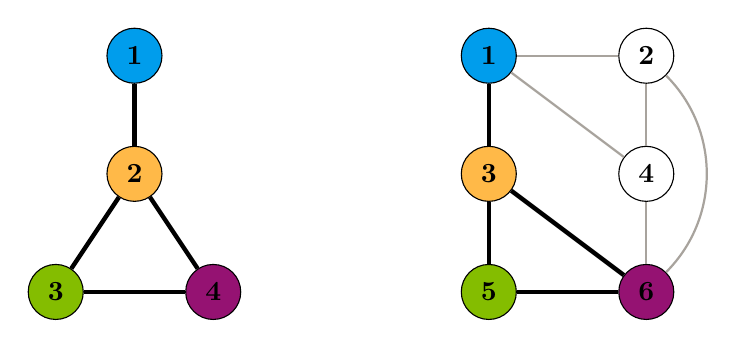
\begin{tikzpicture}
        \node[draw, circle, fill=uofgcobalt, inner sep=4pt, font=\bfseries] (Na) at (1,  0) {1};
        \node[draw, circle, fill=uofgpumpkin, inner sep=4pt, font=\bfseries] (Nb) at (1, -1.5) {2};
        \node[draw, circle, fill=uofglawn, inner sep=4pt, font=\bfseries] (Nc) at (0, -3) {3};
        \node[draw, circle, fill=uofgthistle, inner sep=4pt, font=\bfseries] (Nd) at (2, -3) {4};

        \draw [ultra thick] (Na) -- (Nb);
        \draw [ultra thick] (Nb) -- (Nc);
        \draw [ultra thick] (Nc) -- (Nd);
        \draw [ultra thick] (Nb) -- (Nd);

        \node[draw, circle, fill=uofgcobalt, inner sep=4pt, font=\bfseries] (N1) at (5.5,  0) {1};
        \node[draw, circle, fill=white, inner sep=4pt, font=\bfseries] (N2) at (7.5,  0) {2};
        \node[draw, circle, fill=uofgpumpkin, inner sep=4pt, font=\bfseries] (N3) at (5.5, -1.5) {3};
        \node[draw, circle, fill=white, inner sep=4pt, font=\bfseries] (N4) at (7.5, -1.5) {4};
        \node[draw, circle, fill=uofglawn, inner sep=4pt, font=\bfseries] (N5) at (5.5, -3) {5};
        \node[draw, circle, fill=uofgthistle, inner sep=4pt, font=\bfseries] (N6) at (7.5, -3) {6};

        \draw [thick, color=uofgsandstone!50] (N1) -- (N2);
        \draw [ultra thick] (N1) -- (N3);
        \draw [thick, color=uofgsandstone!50] (N1) -- (N4);
        \draw [thick, color=uofgsandstone!50] (N2) -- (N4);
        \draw [ultra thick] (N3) -- (N5);
        \draw [ultra thick] (N3) -- (N6);
        \draw [thick, color=uofgsandstone!50] (N4) -- (N6);
        \draw [ultra thick] (N5) -- (N6);
        \draw [thick, color=uofgsandstone!50] (N2) to [in=45, out=315] (N6);
    \end{tikzpicture}\end{center}

\end{frame}

\begin{frame}{Maximum Common Subgraph}
    \begin{center}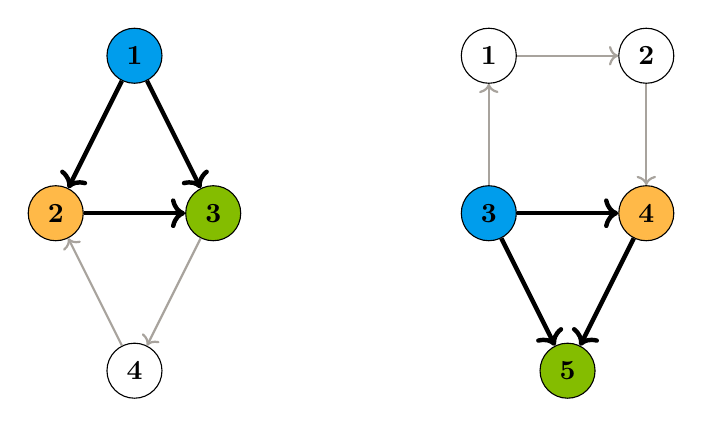
\begin{tikzpicture}%{{{
        \node[draw, circle, fill=uofgcobalt, inner sep=4pt, font=\bfseries] (Ma) at (1, -7.5) {1};
        \node[draw, circle, fill=uofgpumpkin, inner sep=4pt, font=\bfseries] (Mb) at (0, -9.5) {2};
        \node[draw, circle, fill=uofglawn, inner sep=4pt, font=\bfseries] (Mc) at (2, -9.5) {3};
        \node[draw, circle, fill=white, inner sep=4pt, font=\bfseries] (Md) at (1, -11.5) {4};

        \node[draw, circle, fill=white, inner sep=4pt, font=\bfseries] (M1) at (5.5, -7.5) {1};
        \node[draw, circle, fill=white, inner sep=4pt, font=\bfseries] (M2) at (7.5, -7.5) {2};
        \node[draw, circle, fill=uofgcobalt, inner sep=4pt, font=\bfseries] (M3) at (5.5, -9.5) {3};
        \node[draw, circle, fill=uofgpumpkin, inner sep=4pt, font=\bfseries] (M4) at (7.5, -9.5) {4};
        \node[draw, circle, fill=uofglawn, inner sep=4pt, font=\bfseries] (M5) at (6.5, -11.5) {5};

        \draw [->, thick, color=uofgsandstone!50] (Mc) -> (Md);
        \draw [->, thick, color=uofgsandstone!50] (Md) -- (Mb);
        \draw [->, ultra thick] (Ma) -> (Mb);
        \draw [->, ultra thick] (Mb) -> (Mc);
        \draw [->, ultra thick] (Ma) -> (Mc);

        \draw [->, thick, color=uofgsandstone!50] (M1) -> (M2);
        \draw [->, thick, color=uofgsandstone!50] (M2) -> (M4);
        \draw [->, thick, color=uofgsandstone!50] (M3) -> (M1);
        \draw [->, ultra thick] (M3) -> (M4);
        \draw [->, ultra thick] (M3) -> (M5);
        \draw [->, ultra thick] (M4) -> (M5);
    \end{tikzpicture}\end{center}
\end{frame}

\begin{frame}{Maximum Common Connected Subgraph}

    \begin{columns}
        \begin{column}{0.45\textwidth}
            \centering
            \chemfig{*6(-=(-[7]N(-[5]H)(-[7]H))-=-=)}
        \end{column}
        \begin{column}{0.45\textwidth}
            \centering
            \chemfig{*6(-=(-[7]O-[7]N(-[5]H)(-[7]H))-=-=)}
        \end{column}
    \end{columns}

\end{frame}

\section{Solving\ldots}

\begin{frame}{Who Cares?}
    \begin{columns}
        \begin{column}{0.45\textwidth}
            \begin{itemize}
                \item Bioinformatics
                \item Chemistry
                \item Drug design
                \item Computer vision
                \item Pattern recognition
                \item Financial fraud detection
                \item Model checking
                \item Fault detection
            \end{itemize}
        \end{column}
        \begin{column}{0.45\textwidth}
            \begin{itemize}
                \item Law enforcement
                \item Kidney exchange
                \item Social network analysis
                \item Compilers
                \item Diseased cows
                \item Computer algebra
                \item Circuit design
                \item Network design
            \end{itemize}
        \end{column}
    \end{columns}
\end{frame}

\begin{frame}{Practical Algorithms}
    \begin{itemize}
        \item Real-world inputs rarely have nice properties (low treewidth, particular degree
            spreads that are polynomial, etc).

        \item Worst-case performance analysis tells us nothing.

        \item Constant factors matter.
    \end{itemize}
\end{frame}

\begin{frame}{Constraint Models}
    \begin{itemize}
        \item We have some \textbf{variables}, each with a \textbf{domain}, and we want to give each
            variable a value from its domain.
            \begin{itemize}
                \item Clique: a boolean variable for each vertex.
                \item Subgraph isomorphism: a variable for each pattern vertex, with domains being
                    target vertices.
            \end{itemize}
        \item There are \textbf{constraints} between variables.
            \begin{itemize}
                \item Clique: for each pair of non-adjacent vertices, at least one of the two
                    variables must be false.
                \item Subgraph isomorphism: all-different (injectivity), and adjacent pairs of
                    vertices must be mapped to adjacent pairs of vertices.
            \end{itemize}
        \item There is an \textbf{objective}.
            \begin{itemize}
                \item Clique: set as many variables to true as possible.
                \item Subgraph isomorphism: give each variable a value.
            \end{itemize}
    \end{itemize}
\end{frame}

\begin{frame}{Preprocessing}
    \begin{itemize}
        \item We want to \textbf{cross out values} from domains, until only one value is left in
            each.
        \item Subgraph isomorphism: high degree vertices cannot be mapped to low degree vertices.
    \end{itemize}
\end{frame}

\begin{frame}{Search}
    \begin{itemize}
        \item Sometimes we have to \textbf{guess}: pick a variable $x$. Then for each value $v_i$ in
            its domain in turn, see what happens if we force $x = v_i$.
        \item There are good heuristics telling us which variable to pick first.
        \item There are heuristics telling us which value to pick first, but this seems to be
            less reliable in general.
    \end{itemize}
\end{frame}

\begin{frame}{Inference}
    \begin{itemize}
        \item After we guess an assignment, we can \textbf{infer additional deletions}. This can
            have a cascade effect.
    \end{itemize}
\end{frame}

\begin{frame}{Implied Constraints for Subgraph Isomorphism}
    \only<1> {
        \begin{itemize}
            \item Adjacent vertices must be mapped to adjacent vertices.
            \item Vertices that are distance 2 apart must be mapped to vertices that are within
                distance 2.
            \item Vertices that are distance $k$ apart must be mapped to vertices that are within
                distance $k$.
        \end{itemize}

        \vspace{1em}

        \centering
        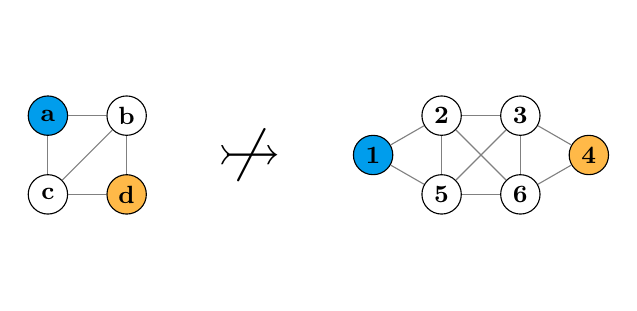
\begin{tikzpicture}
            \node [vertex] (Pc) at (0, 0) { c };
            \node [vertexc3] (Pd) at (1, 0) { d };
            \node [vertex] (Pb) at (1, 1) { b };
            \node [vertexc1] (Pa) at (0, 1) { a };

            \draw [edge] (Pa) -- (Pb);
            \draw [edge] (Pb) -- (Pc);
            \draw [edge] (Pc) -- (Pd);
            \draw [edge] (Pd) -- (Pb);
            \draw [edge] (Pa) -- (Pc);

            \node [anchor=center, font=\huge] at (2.565, 0.5) { $\centernot\rightarrowtail$ };

            \node [vertexc1] (T1) at (4.13, 0.5) { 1 };
            \node [vertex] (T5) at (5, 0) { 5 };
            \node [vertex] (T6) at (6, 0) { 6 };
            \node [vertex] (T3) at (6, 1) { 3 };
            \node [vertex] (T2) at (5, 1) { 2 };
            \node [vertexc3] (T4) at (6.87, 0.5) { 4 };

            \draw [edge] (T1) -- (T2);
            \draw [edge] (T1) -- (T5);
            \draw [edge] (T4) -- (T3);
            \draw [edge] (T4) -- (T6);
            \draw [edge] (T2) -- (T6);
            \draw [edge] (T2) -- (T3);
            \draw [edge] (T3) -- (T5);
            \draw [edge] (T5) -- (T6);
            \draw [edge] (T3) -- (T6);
            \draw [edge] (T2) -- (T5);

            \node at (5, 2) { ~ };
            \node at (5, -1) { ~ };
        \end{tikzpicture}
        \vspace{1em}
    }

    \only<2> {
        \begin{itemize}
            \item $G^d$ is the graph with the same vertex set as $G$, and an edge between $v$ and
                $w$ if the distance between $v$ and $w$ in $G$ is at most $d$.

            \item For any $d$, a subgraph isomorphism $i : P \rightarrowtail T$ is also a
                subgraph isomorphism $i^d : P^d \rightarrowtail T^d$.
        \end{itemize}

        \vspace{1em}

        \centering
        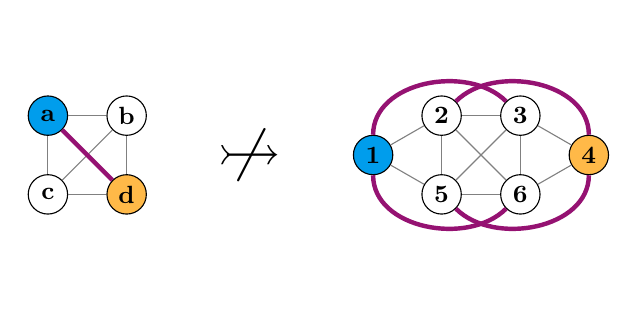
\begin{tikzpicture}
            \node [vertex] (Pc) at (0, 0) { c };
            \node [vertexc3] (Pd) at (1, 0) { d };
            \node [vertex] (Pb) at (1, 1) { b };
            \node [vertexc1] (Pa) at (0, 1) { a };

            \draw [edge] (Pa) -- (Pb);
            \draw [edge] (Pb) -- (Pc);
            \draw [edge] (Pc) -- (Pd);
            \draw [edge] (Pd) -- (Pb);
            \draw [edge] (Pa) -- (Pc);

            \draw [edgel3] (Pa) -- (Pd);

            \node [anchor=center, font=\huge] at (2.565, 0.5) { $\centernot\rightarrowtail$ };

            \node [vertexc1] (T1) at (4.13, 0.5) { 1 };
            \node [vertex] (T5) at (5, 0) { 5 };
            \node [vertex] (T6) at (6, 0) { 6 };
            \node [vertex] (T3) at (6, 1) { 3 };
            \node [vertex] (T2) at (5, 1) { 2 };
            \node [vertexc3] (T4) at (6.87, 0.5) { 4 };

            \draw [edge] (T1) -- (T2);
            \draw [edge] (T1) -- (T5);
            \draw [edge] (T4) -- (T3);
            \draw [edge] (T4) -- (T6);
            \draw [edge] (T2) -- (T6);
            \draw [edge] (T2) -- (T3);
            \draw [edge] (T3) -- (T5);
            \draw [edge] (T5) -- (T6);
            \draw [edge] (T3) -- (T6);
            \draw [edge] (T2) -- (T5);

            \draw [edgel3] (T1) to [in=135, out=90] (T3);
            \draw [edgel3] (T1) to [in=225, out=270] (T6);

            \draw [edgel3] (T4) to [in=45, out=90] (T2);
            \draw [edgel3] (T4) to [in=315, out=270] (T5);

            \node at (5, 2) { ~ };
            \node at (5, -1) { ~ };
        \end{tikzpicture}
        \vspace{1em}
    }

    \only<3> {
        \begin{itemize}
            \item We can do something stronger: rather than looking at distances, we can look at
                \textbf{(simple) paths}, and we can count how many there are.

            \item This is \NP-hard in general, but only lengths 2 and 3 and counts of 2 and 3 are
                useful in practice.

            \item We construct these graph pairs once, at the top of search.
        \end{itemize}
    }

\end{frame}

\begin{frame}{Backtracking Search as a Tree}
    \only<1> {
        \begin{itemize}
            \item Sometimes we guess incorrectly, or there is no solution.
            \item When a variable's domain becomes empty, we fail, and \textbf{backtrack} one level
                and try something else.
        \end{itemize}
    }

    \only<2> {
        \begin{center}
        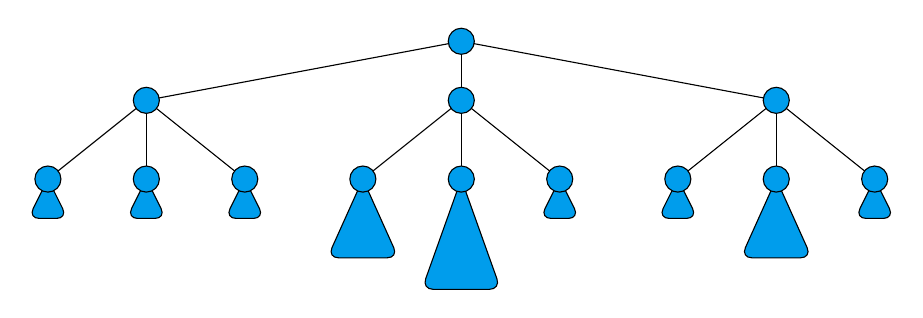
\begin{tikzpicture}%{{{
            \coordinate (R);

            \coordinate (N) at (R);

            \coordinate (N1) at ($(N) + (-4, -0.75)$);
            \coordinate (N2) at ($(N) + ( 0, -0.75)$);
            \coordinate (N3) at ($(N) + ( 4, -0.75)$);

            \foreach \na in {1, ..., 3}{
                \coordinate (N\na 1) at ($(N\na) + (-1.25, -1)$);
                \coordinate (N\na 2) at ($(N\na) + ( 0,    -1)$);
                \coordinate (N\na 3) at ($(N\na) + ( 1.25, -1)$);

                \foreach \nb in {1, ..., 3}{
                    \coordinate (N\na\nb t1) at ($(N\na\nb) + (-0.45, -1)$);
                    \coordinate (N\na\nb t2) at ($(N\na\nb) + ( 0.45, -1)$);

                    \coordinate (N\na\nb s1) at ($(N\na\nb) + (-0.25, -0.5)$);
                    \coordinate (N\na\nb s2) at ($(N\na\nb) + ( 0.25, -0.5)$);

                    \coordinate (N\na\nb h1) at ($(N\na\nb) + (-0.5, -1.4)$);
                    \coordinate (N\na\nb h2) at ($(N\na\nb) + ( 0.5, -1.4)$);
                }
            }

            \foreach \na in {1, ..., 3}{
                \draw (N) -- (N\na);
                \foreach \nb in {1, ..., 3}{
                    \draw (N\na) -- (N\na\nb);
                }
            }

            \tikzstyle{t} = [draw, fill, fill=uofgcobalt, rounded corners];

            \draw [t] (N11) -- (N11s1) -- (N11s2) -- cycle;
            \draw [t] (N12) -- (N12s1) -- (N12s2) -- cycle;
            \draw [t] (N13) -- (N13s1) -- (N13s2) -- cycle;

            \draw [t] (N21) -- (N21t1) -- (N21t2) -- cycle;
            \draw [t] (N22) -- (N22h1) -- (N22h2) -- cycle;
            \draw [t] (N23) -- (N23s1) -- (N23s2) -- cycle;

            \draw [t] (N31) -- (N31s1) -- (N31s2) -- cycle;
            \draw [t] (N32) -- (N32t1) -- (N32t2) -- cycle;
            \draw [t] (N33) -- (N33s1) -- (N33s2) -- cycle;

            \tikzstyle{c} = [draw, circle, fill, fill=uofgcobalt];
            \node [c] at (N) { };

            \foreach \na in {1, ..., 3}{
                \node [c] at (N\na) { };

                \foreach \nb in {1, ..., 3}{
                    \node [c] at (N\na\nb) { };
                }
            }
        \end{tikzpicture}%}}}
        \end{center}
    }

\end{frame}

\begin{frame}{Branch and Bound}

    \begin{center}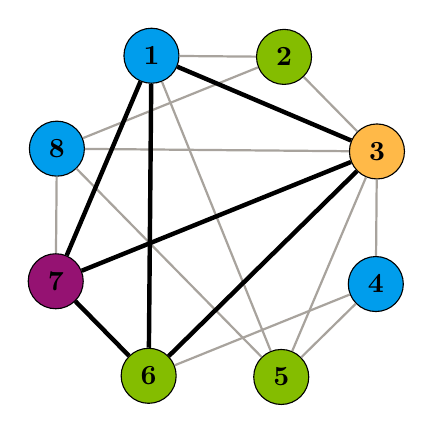
\begin{tikzpicture}
        \newcount \c
        \foreach \n in {1, ..., 8}{
            \c=\n \advance\c by -1 \multiply\c by -360 \divide\c by 8 \advance\c by 112.5
            \ifthenelse{\n = 1 \OR \n = 4 \OR \n = 8}{
                \node[draw, circle, fill=uofgcobalt, inner sep=4pt, font=\bfseries] (N\n) at (\the\c:2.2) {\n};
            }{}
            \ifthenelse{\n = 2 \OR \n = 5 \OR \n = 6}{
                \node[draw, circle, fill=uofglawn, inner sep=4pt, font=\bfseries] (N\n) at (\the\c:2.2) {\n};
            }{}
            \ifthenelse{\n = 3}{
                \node[draw, circle, fill=uofgpumpkin, inner sep=4pt, font=\bfseries] (N\n) at (\the\c:2.2) {\n};
            }{}
            \ifthenelse{\n = 7}{
                \node[draw, circle, fill=uofgthistle, inner sep=4pt, font=\bfseries] (N\n) at (\the\c:2.2) {\n};
            }{}
        }

        \draw [thick, color=uofgsandstone!50] (N1) -- (N2);
        \draw [thick, color=uofgsandstone!50] (N1) -- (N5);
        \draw [thick, color=uofgsandstone!50] (N2) -- (N3);
        \draw [thick, color=uofgsandstone!50] (N2) -- (N8);
        \draw [thick, color=uofgsandstone!50] (N3) -- (N4);
        \draw [thick, color=uofgsandstone!50] (N3) -- (N5);
        \draw [thick, color=uofgsandstone!50] (N3) -- (N8);
        \draw [thick, color=uofgsandstone!50] (N4) -- (N5);
        \draw [thick, color=uofgsandstone!50] (N4) -- (N6);
        \draw [thick, color=uofgsandstone!50] (N5) -- (N8);
        \draw [thick, color=uofgsandstone!50] (N7) -- (N8);

        \draw [ultra thick] (N1) -- (N3);
        \draw [ultra thick] (N1) -- (N6);
        \draw [ultra thick] (N1) -- (N7);
        \draw [ultra thick] (N3) -- (N6);
        \draw [ultra thick] (N3) -- (N7);
        \draw [ultra thick] (N6) -- (N7);
    \end{tikzpicture}\end{center}

    \begin{itemize}
        \item For optimisation: keep track of the \textbf{best solution} we've found so far. If we can show
            we can't beat it, backtrack immediately.
    \end{itemize}

\end{frame}

\begin{frame}{Eliminable Sub-trees}
    \begin{center}
    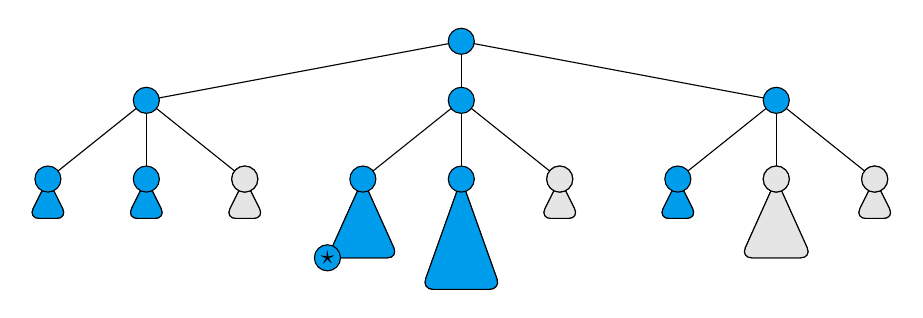
\begin{tikzpicture}%{{{
        \coordinate (R);

        \coordinate (N) at (R);

        \coordinate (N1) at ($(N) + (-4, -0.75)$);
        \coordinate (N2) at ($(N) + ( 0, -0.75)$);
        \coordinate (N3) at ($(N) + ( 4, -0.75)$);

        \foreach \na in {1, ..., 3}{
            \coordinate (N\na 1) at ($(N\na) + (-1.25, -1)$);
            \coordinate (N\na 2) at ($(N\na) + ( 0,    -1)$);
            \coordinate (N\na 3) at ($(N\na) + ( 1.25, -1)$);

            \foreach \nb in {1, ..., 3}{
                \coordinate (N\na\nb t1) at ($(N\na\nb) + (-0.45, -1)$);
                \coordinate (N\na\nb t2) at ($(N\na\nb) + ( 0.45, -1)$);

                \coordinate (N\na\nb s1) at ($(N\na\nb) + (-0.25, -0.5)$);
                \coordinate (N\na\nb s2) at ($(N\na\nb) + ( 0.25, -0.5)$);

                \coordinate (N\na\nb h1) at ($(N\na\nb) + (-0.5, -1.4)$);
                \coordinate (N\na\nb h2) at ($(N\na\nb) + ( 0.5, -1.4)$);
            }
        }

        \foreach \na in {1, ..., 3}{
            \draw (N) -- (N\na);
            \foreach \nb in {1, ..., 3}{
                \draw (N\na) -- (N\na\nb);
            }
        }

        \tikzstyle{t} = [draw, fill, fill=uofgcobalt, rounded corners];
        \tikzstyle{u} = [draw, fill, fill=black!10!white, rounded corners];

        \draw <1> [t] (N11) -- (N11s1) -- (N11s2) -- cycle;
        \draw <1> [t] (N12) -- (N12s1) -- (N12s2) -- cycle;
        \draw <1> [t] (N13) -- (N13s1) -- (N13s2) -- cycle;
        \draw <1> [t] (N21) -- (N21t1) -- (N21t2) -- cycle;
        \draw <1> [t] (N22) -- (N22h1) -- (N22h2) -- cycle;
        \draw <1> [t] (N23) -- (N23s1) -- (N23s2) -- cycle;
        \draw <1> [t] (N31) -- (N31s1) -- (N31s2) -- cycle;
        \draw <1> [t] (N32) -- (N32t1) -- (N32t2) -- cycle;
        \draw <1> [t] (N33) -- (N33s1) -- (N33s2) -- cycle;


        \draw <2> [t] (N11) -- (N11s1) -- (N11s2) -- cycle;
        \draw <2> [t] (N12) -- (N12s1) -- (N12s2) -- cycle;
        \draw <2> [u] (N13) -- (N13s1) -- (N13s2) -- cycle;
        \draw <2> [t] (N21) -- (N21t1) -- (N21t2) -- cycle;
        \draw <2> [t] (N22) -- (N22h1) -- (N22h2) -- cycle;
        \draw <2> [u] (N23) -- (N23s1) -- (N23s2) -- cycle;
        \draw <2> [t] (N31) -- (N31s1) -- (N31s2) -- cycle;
        \draw <2> [u] (N32) -- (N32t1) -- (N32t2) -- cycle;
        \draw <2> [u] (N33) -- (N33s1) -- (N33s2) -- cycle;

        \tikzstyle{c} = [draw, circle, fill, fill=uofgcobalt];
        \tikzstyle{d} = [draw, circle, fill, fill=black!10!white];
        \node [c] at (N) { };

        \foreach \na in {1, ..., 3}{
            \node [c] at (N\na) { };

            \foreach \nb in {1, ..., 3}{
                \ifthenelse{\nb = 3 \OR \na\nb = 32}{
                    \node <1> [c] at (N\na\nb) { };
                    \node <2> [d] at (N\na\nb) { };
                }{
                    \node [c] at (N\na\nb) { };
                }
            }
        }

        \node [c] at (N21t1) { };
        \node at (N21t1) { $\star$ };
    \end{tikzpicture}%}}}
    \end{center}

\end{frame}

\begin{frame}{Backjumping}

    \begin{itemize}
        \item When backtracking, see if the current assignment actually removed any values which
            could have helped prevent the failure. If not, \textbf{jump back} another step.
    \end{itemize}

\end{frame}

\begin{frame}{Backjumping as a Tree}
    \centering
    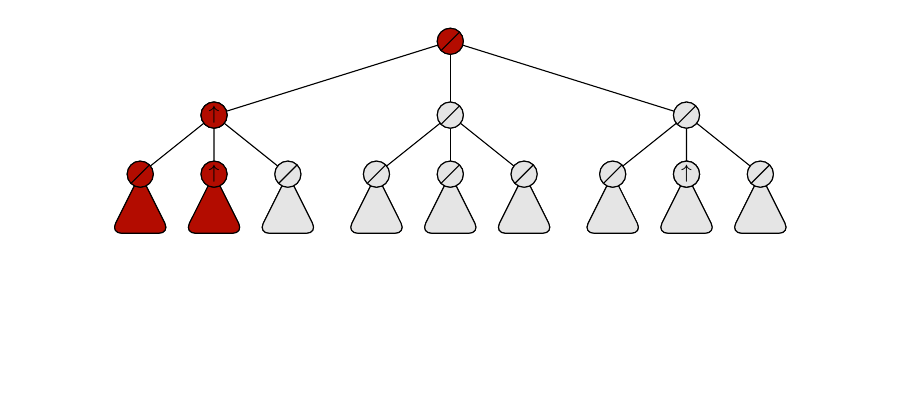
\begin{tikzpicture}[scale=0.75]%{{{
        \coordinate (R);

        \coordinate (N) at (R);

        \coordinate (N1) at ($(N) + (-4, -1.25)$);
        \coordinate (N2) at ($(N) + ( 0, -1.25)$);
        \coordinate (N3) at ($(N) + ( 4, -1.25)$);

        \foreach \na in {1, ..., 3}{
            \coordinate (N\na 1) at ($(N\na) + (-1.25, -1)$);
            \coordinate (N\na 2) at ($(N\na) + ( 0,    -1)$);
            \coordinate (N\na 3) at ($(N\na) + ( 1.25, -1)$);

            \foreach \nb in {1, ..., 3}{
                \coordinate (N\na\nb t1) at ($(N\na\nb) + (-0.5, -1)$);
                \coordinate (N\na\nb t2) at ($(N\na\nb) + ( 0.5, -1)$);

                \coordinate (N\na\nb s1) at ($(N\na\nb) + (-0.3, -0.6)$);
                \coordinate (N\na\nb s2) at ($(N\na\nb) + ( 0.3, -0.6)$);

                \coordinate (N\na\nb h1) at ($(N\na\nb) + (-1.5, -3)$);
                \coordinate (N\na\nb h2) at ($(N\na\nb) + ( 1.5, -3)$);
            }
        }

        \foreach \na in {1, ..., 3}{
            \draw (N) -- (N\na);
            \foreach \nb in {1, ..., 3}{
                \draw (N\na) -- (N\na\nb);
            }
        }

        \tikzstyle{t} = [draw, fill, fill=uofgcobalt, rounded corners];
        \tikzstyle{tf} = [draw, fill, fill=uofgpillarbox, rounded corners];
        \tikzstyle{ts} = [draw, fill, fill=black!10!white, rounded corners];
        \foreach \na in {1, ..., 3}{
            \foreach \nb in {1, ..., 3}{
                \ifthenelse{\na = 1}{
                    \ifthenelse{\na\nb = 11}{
                        \draw <1> [t] (N\na\nb) -- (N\na\nb t1) -- (N\na\nb t2) -- cycle;
                        \draw <2-> [tf] (N\na\nb) -- (N\na\nb t1) -- (N\na\nb t2) -- cycle;
                    }{}
                    \ifthenelse{\na\nb = 12}{
                        \draw <1-2> [t] (N\na\nb) -- (N\na\nb t1) -- (N\na\nb t2) -- cycle;
                        \draw <3-> [tf] (N\na\nb) -- (N\na\nb t1) -- (N\na\nb t2) -- cycle;
                    }{}
                    \ifthenelse{\na\nb = 13}{
                        \draw <1-3> [t] (N\na\nb) -- (N\na\nb t1) -- (N\na\nb t2) -- cycle;
                        \draw <4-> [ts] (N\na\nb) -- (N\na\nb t1) -- (N\na\nb t2) -- cycle;
                    }{}
                }{
                    \draw <1-6> [t] (N\na\nb) -- (N\na\nb t1) -- (N\na\nb t2) -- cycle;
                    \draw <7-> [ts] (N\na\nb) -- (N\na\nb t1) -- (N\na\nb t2) -- cycle;
                }
            }
        }

        \tikzstyle{c} = [draw, circle, fill, fill=uofgcobalt];
        \tikzstyle{cf} = [draw, circle, fill, fill=uofgpillarbox];
        \tikzstyle{cx} = [draw, forbidden sign, fill, fill=uofgpillarbox];
        \tikzstyle{cs} = [draw, forbidden sign, fill, fill=black!10!white];
        \tikzstyle{cfs} = [draw, circle, fill, fill=black!10!white];
        \node <1-7> [c] at (N) { };
        \node <8-> [cx] at (N) { };

        \foreach \na in {1, ..., 3}{
            \ifthenelse{\na = 1}{
                \node <1-4> [c] at (N\na) { };
                \node <5> [cx] at (N\na) { };
                \node <6-> [cf] at (N\na) { };
                \node <6-> [font=\scriptsize] at (N1) { $\uparrow$ };
            }{
                \node <1-6> [c] at (N\na) { };
                \node <7-> [cs] at (N\na) { };
            }

            \foreach \nb in {1, ..., 3}{
                \ifthenelse{\na = 1}{
                    \ifthenelse{\na\nb = 11}{
                        \node <1> [c] at (N\na\nb) { };
                        \node <2-> [cx] at (N\na\nb) { };
                    }{}
                    \ifthenelse{\na\nb = 12}{
                        \node <1-2> [c] at (N\na\nb) { };
                        \node <3-> [cf] at (N\na\nb) { };
                        \node <3-> [font=\scriptsize] at (N12) { $\uparrow$ };
                    }{}
                    \ifthenelse{\na\nb = 13}{
                        \node <1-3> [c] at (N\na\nb) { };
                        \node <4-> [cs] at (N\na\nb) { };
                    }{}
                }{
                    \node <1-6> [c] at (N\na\nb) { };

                    \ifthenelse{\na\nb = 32}{
                        \node <7-8> [cs] at (N\na\nb) { };
                        \node <9-> [cfs] at (N\na\nb) { };
                        \node <9-> [font=\scriptsize] at (N32) { $\uparrow$ };
                    }{
                        \node <7-> [cs] at (N\na\nb) { };
                    }
                }
            }
        }

        \node at (-7, -5.5) { }; \node at (7, -5.5) { };
    \end{tikzpicture}%}}}
\end{frame}

\section{\ldots{}In Parallel}

\begin{frame}{Thread-Parallel Tree Search}

    \only<1-3> {
        \centering
        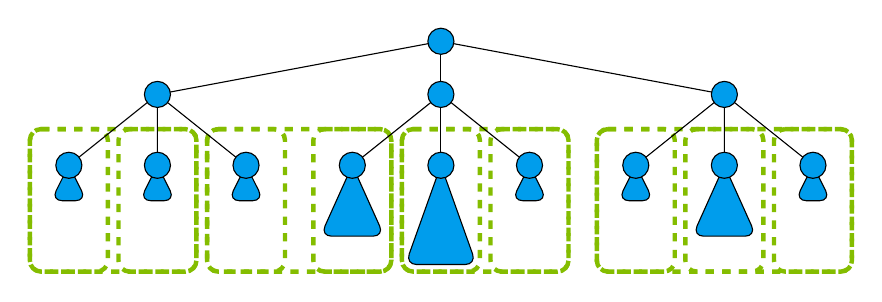
\begin{tikzpicture}[scale=0.9]%{{{
            \coordinate (R);

            \coordinate (N) at (R);

            \coordinate (N1) at ($(N) + (-4, -0.75)$);
            \coordinate (N2) at ($(N) + ( 0, -0.75)$);
            \coordinate (N3) at ($(N) + ( 4, -0.75)$);

            \foreach \na in {1, ..., 3}{
                \coordinate (N\na 1) at ($(N\na) + (-1.25, -1)$);
                \coordinate (N\na 2) at ($(N\na) + ( 0,    -1)$);
                \coordinate (N\na 3) at ($(N\na) + ( 1.25, -1)$);

                \foreach \nb in {1, ..., 3}{
                    \coordinate (N\na\nb t1) at ($(N\na\nb) + (-0.45, -1)$);
                    \coordinate (N\na\nb t2) at ($(N\na\nb) + ( 0.45, -1)$);

                    \coordinate (N\na\nb s1) at ($(N\na\nb) + (-0.25, -0.5)$);
                    \coordinate (N\na\nb s2) at ($(N\na\nb) + ( 0.25, -0.5)$);

                    \coordinate (N\na\nb h1) at ($(N\na\nb) + (-0.5, -1.4)$);
                    \coordinate (N\na\nb h2) at ($(N\na\nb) + ( 0.5, -1.4)$);
                }
            }

            \tikzstyle{i} = [draw, rounded corners, dashed, color=white, ultra thick];
            \draw <1> [i] ($(N11) + (-0.55, 0.51)$) -- ($(N12) + (0.55, 0.51)$) -- ($(N12) + (0.55, -1.5)$) -- ($(N11) + (-0.55, -1.5)$) -- cycle;
            \draw <1> [i] ($(N13) + (-0.55, 0.51)$) -- ($(N21) + (0.55, 0.51)$) -- ($(N21) + (0.55, -1.5)$) -- ($(N13) + (-0.55, -1.5)$) -- cycle;
            \draw <1> [i] ($(N22) + (-0.55, 0.51)$) -- ($(N23) + (0.55, 0.51)$) -- ($(N23) + (0.55, -1.5)$) -- ($(N22) + (-0.55, -1.5)$) -- cycle;
            \draw <1> [i] ($(N31) + (-0.55, 0.51)$) -- ($(N33) + (0.55, 0.51)$) -- ($(N33) + (0.55, -1.5)$) -- ($(N31) + (-0.55, -1.5)$) -- cycle;

            \tikzstyle{p} = [draw, rounded corners, dashed, color=uofglawn, ultra thick];
            \draw <2> [p] ($(N11) + (-0.55, 0.51)$) -- ($(N12) + (0.55, 0.51)$) -- ($(N12) + (0.55, -1.5)$) -- ($(N11) + (-0.55, -1.5)$) -- cycle;
            \draw <2> [p] ($(N13) + (-0.55, 0.51)$) -- ($(N21) + (0.55, 0.51)$) -- ($(N21) + (0.55, -1.5)$) -- ($(N13) + (-0.55, -1.5)$) -- cycle;
            \draw <2> [p] ($(N22) + (-0.55, 0.51)$) -- ($(N23) + (0.55, 0.51)$) -- ($(N23) + (0.55, -1.5)$) -- ($(N22) + (-0.55, -1.5)$) -- cycle;
            \draw <2> [p] ($(N31) + (-0.55, 0.51)$) -- ($(N33) + (0.55, 0.51)$) -- ($(N33) + (0.55, -1.5)$) -- ($(N31) + (-0.55, -1.5)$) -- cycle;

            \foreach \na in {1, ..., 3}{
                \foreach \nb in {1, ..., 3}{
                    \draw <3> [p] ($(N\na\nb) + (-0.55, 0.51)$) -- ($(N\na\nb) + (0.55, 0.51)$) --
                    ($(N\na\nb) + (0.55, -1.5)$) -- ($(N\na\nb) + (-0.55, -1.5)$) -- cycle;
                }
            }

            \foreach \na in {1, ..., 3}{
                \draw (N) -- (N\na);
                \foreach \nb in {1, ..., 3}{
                    \draw (N\na) -- (N\na\nb);
                }
            }

            \tikzstyle{t} = [draw, fill, fill=uofgcobalt, rounded corners];

            \draw [t] (N11) -- (N11s1) -- (N11s2) -- cycle;
            \draw [t] (N12) -- (N12s1) -- (N12s2) -- cycle;
            \draw [t] (N13) -- (N13s1) -- (N13s2) -- cycle;

            \draw [t] (N21) -- (N21t1) -- (N21t2) -- cycle;
            \draw [t] (N22) -- (N22h1) -- (N22h2) -- cycle;
            \draw [t] (N23) -- (N23s1) -- (N23s2) -- cycle;

            \draw [t] (N31) -- (N31s1) -- (N31s2) -- cycle;
            \draw [t] (N32) -- (N32t1) -- (N32t2) -- cycle;
            \draw [t] (N33) -- (N33s1) -- (N33s2) -- cycle;

            \tikzstyle{c} = [draw, circle, fill, fill=uofgcobalt];
            \node [c] at (N) { };

            \foreach \na in {1, ..., 3}{
                \node [c] at (N\na) { };

                \foreach \nb in {1, ..., 3}{
                    \node [c] at (N\na\nb) { };
                }
            }
        \end{tikzpicture}%}}}
    }

\end{frame}

\begin{frame}{Parallel Search Order Matters}

    \only<1-2> {
        \centering
        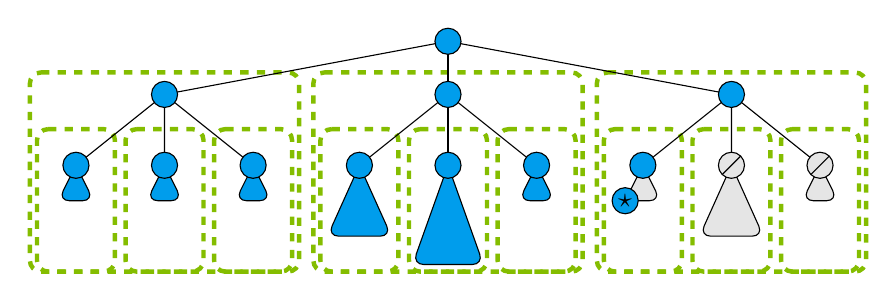
\begin{tikzpicture}[scale=0.9]%{{{
            \coordinate (R);

            \coordinate (N) at (R);

            \coordinate (N1) at ($(N) + (-4, -0.75)$);
            \coordinate (N2) at ($(N) + ( 0, -0.75)$);
            \coordinate (N3) at ($(N) + ( 4, -0.75)$);


            \foreach \na in {1, ..., 3}{
                \coordinate (N\na 1) at ($(N\na) + (-1.25, -1)$);
                \coordinate (N\na 2) at ($(N\na) + ( 0,    -1)$);
                \coordinate (N\na 3) at ($(N\na) + ( 1.25, -1)$);

                \foreach \nb in {1, ..., 3}{
                    \coordinate (N\na\nb t1) at ($(N\na\nb) + (-0.45, -1)$);
                    \coordinate (N\na\nb t2) at ($(N\na\nb) + ( 0.45, -1)$);

                    \coordinate (N\na\nb s1) at ($(N\na\nb) + (-0.25, -0.5)$);
                    \coordinate (N\na\nb s2) at ($(N\na\nb) + ( 0.25, -0.5)$);

                    \coordinate (N\na\nb h1) at ($(N\na\nb) + (-0.5, -1.4)$);
                    \coordinate (N\na\nb h2) at ($(N\na\nb) + ( 0.5, -1.4)$);
                }
            }

            \tikzstyle{p} = [draw, rounded corners, dashed, color=uofglawn, ultra thick];
            \tikzstyle{q} = [draw, rounded corners, dashed, color=uofglawn, ultra thick];

            \foreach \na in {1, ..., 3}{
                \foreach \nb in {1, ..., 3}{
                    \draw <1> [p] ($(N\na\nb) + (-0.55, 0.51)$) -- ($(N\na\nb) + (0.55, 0.51)$) --
                    ($(N\na\nb) + (0.55, -1.5)$) -- ($(N\na\nb) + (-0.55, -1.5)$) -- cycle;
                }

                \draw <2> [q] ($(N\na 1) + (-0.65, 1.31)$) -- ($(N\na 3) + (0.65, 1.31)$) --
                ($(N\na 3) + (0.65, -1.5)$) -- ($(N\na 1) + (-0.65, -1.5)$) -- cycle;
            }

            \foreach \na in {1, ..., 3}{
                \draw (N) -- (N\na);
                \foreach \nb in {1, ..., 3}{
                    \draw (N\na) -- (N\na\nb);
                }
            }

            \tikzstyle{t} = [draw, fill, fill=uofgcobalt, rounded corners];
            \tikzstyle{u} = [draw, fill, fill=black!10!white, rounded corners];

            \draw [t] (N11) -- (N11s1) -- (N11s2) -- cycle;
            \draw [t] (N12) -- (N12s1) -- (N12s2) -- cycle;
            \draw [t] (N13) -- (N13s1) -- (N13s2) -- cycle;

            \draw [t] (N21) -- (N21t1) -- (N21t2) -- cycle;
            \draw [t] (N22) -- (N22h1) -- (N22h2) -- cycle;
            \draw [t] (N23) -- (N23s1) -- (N23s2) -- cycle;

            \draw [u] (N31) -- (N31s1) -- (N31s2) -- cycle;
            \draw [u] (N32) -- (N32t1) -- (N32t2) -- cycle;
            \draw [u] (N33) -- (N33s1) -- (N33s2) -- cycle;

            \tikzstyle{c} = [draw, circle, fill, fill=uofgcobalt];
            \tikzstyle{e} = [draw, forbidden sign, fill, fill=black!10!white];
            \node [c] at (N) { };

            \foreach \na in {1, ..., 3}{
                \node [c] at (N\na) { };

                \foreach \nb in {1, ..., 3}{
                    \ifthenelse{\na = 1 \OR \na = 2 \OR \na\nb = 31}{
                        \node [c] at (N\na\nb) { };
                    }{
                        \node [e] at (N\na\nb) { };
                    }
                }
            }

            \node [c] at (N31s1) { };
            \node at (N31s1) { $\star$ };
        \end{tikzpicture}%}}}
    }

    \only<3> {
        \centering
        \input{gen-graph-speedup}
    }

    \only <4> {
        \begin{itemize}
            \item Value-ordering heuristics tend to be \textbf{worst high up} the search tree.
            \item But depth-first searches commit completely to the first choice made\ldots
            \item Discrepancy searches can avoid this problem by doing more work in total. Parallel
                search can give \textbf{similar benefits for free}.
        \end{itemize}
    }
\end{frame}

\begin{frame}{Safety and Reproducibility}

    \begin{itemize}
        \item My ``wish list'':
            \begin{enumerate}
                \item Parallel search should not be substantially slower than sequential search.
                \item Adding more processors should not make things substantially worse.
                \item Running the same program twice on the same hardware should give similar
                    runtimes.
            \end{enumerate}
        \item This is surprisingly tricky.
        \item On top of all that, we want to prioritise work stealing from where we're most likely
            to be wrong, or possibly from where we're most likely not to eliminate a subtree.
    \end{itemize}

\end{frame}

\begin{frame}{Parallel Backjumping as a Lazy Fold}

    \only <1> {
        \begin{itemize}
            \item Lazily map each subproblem to Jump $F$ $\KwSty{or}$ Fail $F$ $\KwSty{or}$ Success.
            \item Lazily fold, starting with Fail $\{ v \}$, as follows:
                \begin{alignat*}{2}
                    \underline{\hspace{1em}} &~\circled{$>$}~ \textnormal{Success} \hspace{1em} &&= \textnormal{Success} \\
                    \underline{\hspace{1em}} &~\circled{$>$}~ \textnormal{Jump}~F \hspace{1em} &&= \textnormal{Jump}~F \\
                    \textnormal{Fail}~F &~\circled{$>$}~ \textnormal{Fail}~G \hspace{1em} &&= \textnormal{Fail}~(F \cup G)
                \end{alignat*}
            \item If a Jump $F$ occurs to the left of a Success, we have a bug.
        \end{itemize}
    }

    \only <2> {
        \begin{itemize}
            \item When multiplying, if any item is 0, the result is 0.
                \begin{alignat*}{2}
                    \underline{\hspace{1em}} &~\times~ 0 \hspace{1em} &&= 0 \\
                    0 &~\times~ \underline{\hspace{1em}} \hspace{1em} &&= 0
                \end{alignat*}
            \item Here, if any item is Success, the result is Success, and we do not need to evaluate
                the rest of the map.
                \begin{alignat*}{2}
                    \underline{\hspace{1em}} &~\circled{$>$}~ \textnormal{Success} \hspace{1em} &&= \textnormal{Success}
                \end{alignat*}
            \item If any item is Jump $F$, the result is either Jump $F$, or some Jump $G$ or Success
                that is further to the left. We do not need to evaluate any item to the right.
                \begin{alignat*}{2}
                    \underline{\hspace{1em}} &~\circled{$>$}~ \textnormal{Jump}~F \hspace{1em} &&= \textnormal{Jump}~F
                \end{alignat*}
        \end{itemize}
    }

\end{frame}

\begin{frame}{Parallel Search is Worth Doing}

    \vskip-5pt \input{gen-graph-speedups-scatter}

\end{frame}

\section{Works in Progress}

\begin{frame}{Describing and Implementing Parallel Search}

    \begin{itemize}
        \item Implementing safe and reproducible parallel search by hand, even just for multi-core,
            is painful.
        \item Current high level approaches don't offer the properties we need.
        \item Is there a better way?
    \end{itemize}

\end{frame}

\begin{frame}{Symmetries}

    \begin{itemize}
        \item Some graphs have known symmetries. Can we exploit this?

            \begin{itemize}
                \item In some ways, maximum clique is just a completely symmetric version of maximum
                    common subgraph.
            \end{itemize}

        \item What about if we have to detect the symmetries ourselves dynamically?
    \end{itemize}

\end{frame}

\begin{frame}{Explaining Failures}

    \begin{itemize}
        \item Backjumping works because when we fail, we work out why, and use that to backtrack
            further.

        \item But then we throw that information away\ldots
    \end{itemize}

\end{frame}

\begin{frame}{Generating Hard Subgraph Isomorphism Instances}

    \begin{itemize}
        \item We can solve some random problem instances with a thousand pattern vertices, and ten
            thousand target vertices. Can we solve \emph{any} instance with these sizes?

        \item We like having lots of instances, to make sure we don't overfit algorithm parameters.

        \item How do we randomly create subgraph isomorphism instances?
    \end{itemize}

\end{frame}

\begin{frame}[t]{Phase Transitions}

    \only<1> {
        \input{gen-graph-phase-transition}
    }

    \only<2> {
        \input{gen-graph-non-induced-1}
    }

    \only<3> {
        \input{gen-graph-induced-1}
    }

    \only<4> {
        \input{gen-graph-non-induced-2}
    }

    \only<5> {
        \input{gen-graph-induced-2}
    }

\end{frame}

\begin{frame}{Graph Algorithms and Optimisation}

    \begin{itemize}
        \item How do we solve problems that are ``subgraph isomorphism plus some other
            constraints''?
    \end{itemize}

\end{frame}

\begin{frame}[plain,noframenumbering,b]
    \begin{tikzpicture}[remember picture, overlay]
        \node at (current page.north west) {
            \begin{tikzpicture}[remember picture, overlay]
                \fill [fill=uofguniversityblue, anchor=north west] (0, 0) rectangle (\paperwidth, -1.7cm);
            \end{tikzpicture}
        };

        \node (logo) [anchor=north east, shift={(-0.3cm,-0.2cm)}] at (current page.north east) {
            \includegraphics*[keepaspectratio=true,scale=0.55]{UoG_keyline.pdf}
        };
    \end{tikzpicture}

    \begin{center}
        \url{http://dcs.gla.ac.uk/~ciaran} \\
        \href{mailto:c.mccreesh.1@research.gla.ac.uk}{\nolinkurl{c.mccreesh.1@research.gla.ac.uk}}
        \\ [1cm]
    \end{center}
\end{frame}

\end{document}

